\chapter{Diseño e implementación} % Main chapter title

\label{Chapter3} % Change X to a consecutive number; for referencing this chapter elsewhere, use \ref{ChapterX}

En este capítulo se describe el diseño e implementación del sistema desarrollado que automatiza la toma de datos de las flores de duraznero a través de fotos de varetas.

\section{Arquitectura del sistema}

El sistema general implementado en este trabajo se presenta en la figura \ref{fig:sistemaGeneral}. Este sistema cuenta con un \textit{frontend} donde el usuario sube una foto de vareta de duraznero y posteriormente esta imagen pasará por dos módulos de forma secuencial. El primer módulo, es el encargado de medir la longitud de la vareta y el segundo módulo se encarga de detectar el estado fenológico, la cantidad de flores y el tipo de flores que posee la vareta. Cada uno de los resultados obtenidos por estos módulos es presentado por pantalla al usuario y con la posibilidad de descargarlos en formato CSV.

\begin{figure}[ht]
	\centering
	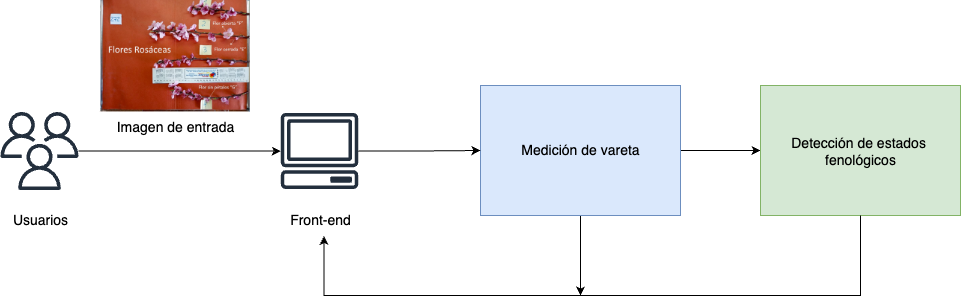
\includegraphics[scale=.4]{./Figures/arq1.drawio.png}
	\caption{Arquitectura general del sistema.}
	\label{fig:sistemaGeneral}
\end{figure}

La arquitectura del módulo que estima la longitud de la vareta se puede observar en la figura \ref{fig:varetaSize}. Este módulo toma y preprocesa la imagen de entrada, posteriormente detecta la regla que es el objeto de referencia y procede a tomar las mediciones en píxeles de dicho elemento. Luego, se hace una conversión de píxeles a centímetros. Una vez finalizada la conversión, se detectan las varetas presentes en la imagen y se calculan sus dimensiones, se revisa la orientación de la foto y se toma la longitud de cada vareta en píxeles. Finalmente, con la conversión anterior se pasa a centímetros las mediciones de las varetas, se anotan los resultados en una tabla y son enviados al siguiente modulo. Por otro lado, la imagen con las mediciones se muestra por pantalla.

Este módulo se detalla con más a profundidad en este mismo capítulo.

\begin{figure}[htpb]
	\centering
	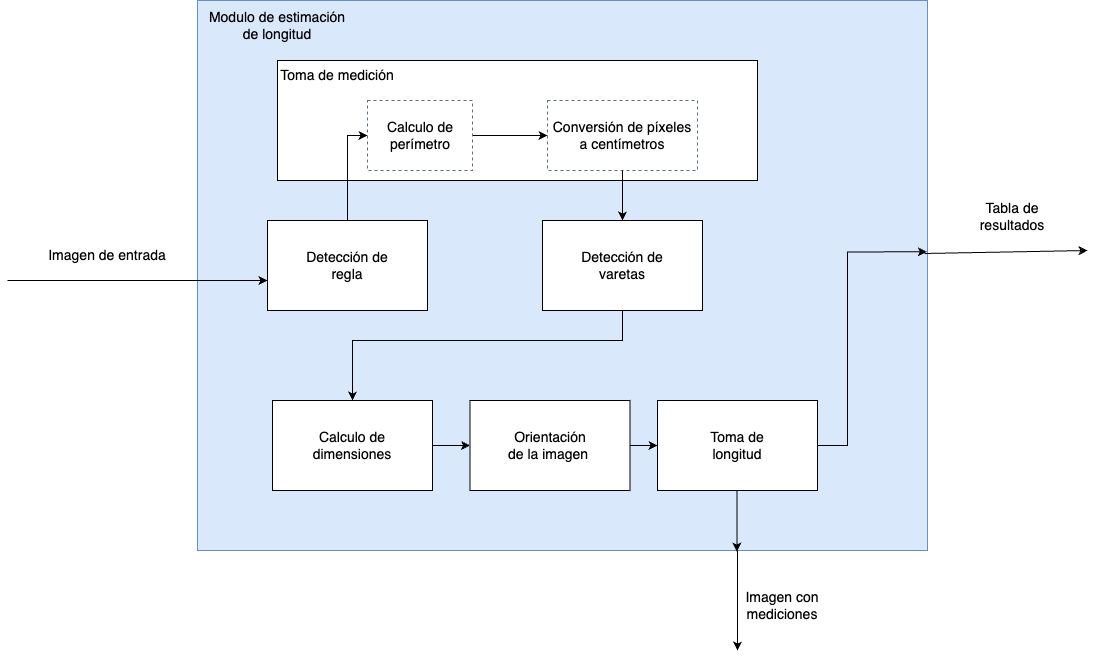
\includegraphics[scale=.4]{./Figures/medicionVareta.drawio.png}
	\caption{Módulo de estimación de longitud.}
	\label{fig:varetaSize}
\end{figure}

La arquitectura del módulo de detección y procesamiento se presenta en la figura \ref{fig:densidadDeFlores}. La entrada a este módulo es la imagen original donde se le aplica un preprocesamiento y posteriormente se pasa por un modelo que detecta los estados fenológicos de las flores de duraznero y sus varetas. Luego, se realiza un postprocesamiento de los resultados para conocer el número de flores totales que se encuentran en la imagen y un conteo de las mismas por vareta. Por último, se extraen las flores detectadas por vareta y son enviadas al clasificador para determinar su tipo.

Más adelante en este mismo capítulo se dará más información detallada de este módulo y de otros bloques del sistema que cumplen una función importante para generar los resultados deseados.

Cabe destacar que la realización de este sistema se llevó a cabo en el lenguaje de programación \textit{Python} y se encuentra diseñado para funcionar en una computadora local bajo un ambiente virtualizado. 

\begin{figure}[htp]
	\centering
	\includegraphics[scale=.35]{./Figures/DetecciónFlor.drawio.png}
	\caption{Módulo de detección y procesamiento.}
	\label{fig:densidadDeFlores}
\end{figure}

\section{Preparación de los datos}

La preparación de los datos es una de las partes más criticas durante el desarrollo de un modelo de aprendizaje. Esto debido a que si los datos no se encuentran en las condiciones adecuadas para su uso en un modelo de IA, el modelo no tendrá un buen rendimiento. 

El presente trabajo requirió la generación de distintos etiquetados para el \textit{dataset} original, debido a la cantidad de modelos utilizados durante su desarrollo.

\subsection{Análisis exploratorio}
El \textit{dataset} original provisto por el INTA contiene las características que se indican en la tabla \ref{tab:flores}. En general, las fotos presentan distintas dimensiones y orientaciones (vertical u horizontal). Por otro lado, se desconoce el tipo de cámara utilizada y el ángulo siempre es cenital.


\begin{table}[h]
	\centering
	\caption[caption corto]{Características de las fotos de duraznos}
	\begin{tabular}{c c c l}    
		\toprule
		\textbf{Formato}     & \textbf{Cantidad} & \textbf{Resolución} & \textbf{Observaciones}\\
		\midrule
		JPG                  & 288               &  Variable &  Cuatro varetas por foto.\\		
		\bottomrule
		\hline
	\end{tabular}
	\label{tab:flores}
\end{table}
 
Las imágenes tienen un fondo naranja y en ocasiones contienen partes grises. Esto debido a que las varetas de duraznero fueron posadas sobre una cartulina color naranja y a veces por las dimensiones de las varetas, estás sobresalen de la cartulina tomando parte de la mesa color gris.

Por otro lado, las fotos presentan cambios de brillo e iluminación, generando distintas tonalidades de los colores de fondo y de flores. 

Los elementos que se observan generalmente en las fotos provistas por el cliente incluyen una regla, cuatro varetas, cartulina de fondo, etiquetas que identifican las varetas y en ocasiones objetos que no forman parte de la detección o que no aportan información.

En la figura \ref{fig:three graphs}, se puede observar algunos ejemplos de fotos con las características que se describieron anteriormente.

\begin{figure}[!htpb]
     \centering
     \begin{subfigure}[b]{0.3\textwidth}
         \centering
         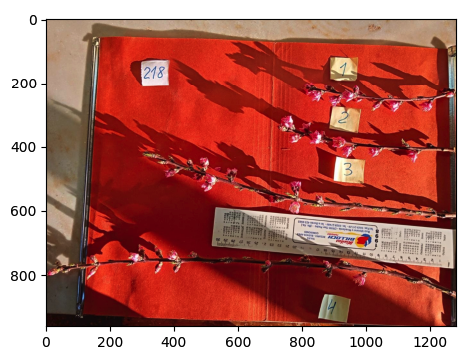
\includegraphics[scale=.3]{./Figures/flor_muestra5.png}
         \caption{Foto de muestra 1.}
         \label{fig:1de3}
     \end{subfigure}
     \hfill
     \begin{subfigure}[b]{0.3\textwidth}
         \centering
         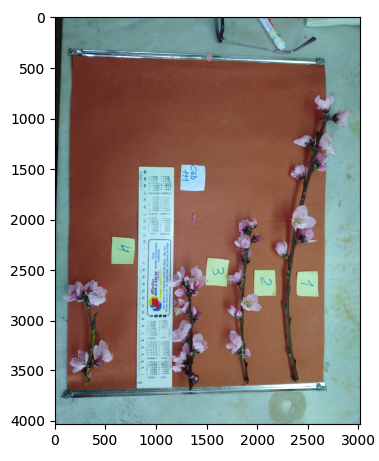
\includegraphics[scale=.35]{./Figures/flor_muestra3.png}
         \caption{Foto de muestra 2.}
         \label{fig:2de3}
     \end{subfigure}
     \hfill
     \begin{subfigure}[b]{0.3\textwidth}
         \centering
         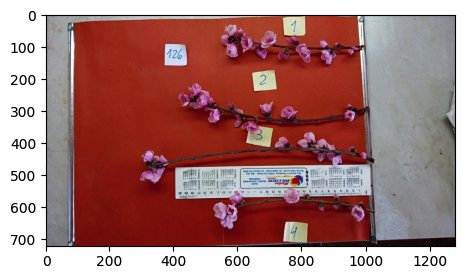
\includegraphics[scale=.35]{./Figures/flor_muestra6.png}
         \caption{Foto de muestra 3.}
         \label{fig:3de3}
     \end{subfigure}
        \caption{Fotos de muestra del conjunto de datos.}
        \label{fig:three graphs}
\end{figure}


 
%\definecolor{mygreen}{rgb}{0,0.6,0}
%\definecolor{mygray}{rgb}{0.5,0.5,0.5}
%\definecolor{mymauve}{rgb}{0.58,0,0.82}
%
%%%%%%%%%%%%%%%%%%%%%%%%%%%%%%%%%%%%%%%%%%%%%%%%%%%%%%%%%%%%%%%%%%%%%%%%%%%%%%
%% parámetros para configurar el formato del código en los entornos lstlisting
%%%%%%%%%%%%%%%%%%%%%%%%%%%%%%%%%%%%%%%%%%%%%%%%%%%%%%%%%%%%%%%%%%%%%%%%%%%%%%
%\lstset{ %
%  backgroundcolor=\color{white},   % choose the background color; you must add \usepackage{color} or \usepackage{xcolor}
%  basicstyle=\footnotesize,        % the size of the fonts that are used for the code
%  breakatwhitespace=false,         % sets if automatic breaks should only happen at whitespace
%  breaklines=true,                 % sets automatic line breaking
%  captionpos=b,                    % sets the caption-position to bottom
%  commentstyle=\color{mygreen},    % comment style
%  deletekeywords={...},            % if you want to delete keywords from the given language
%  %escapeinside={\%*}{*)},          % if you want to add LaTeX within your code
%  %extendedchars=true,              % lets you use non-ASCII characters; for 8-bits encodings only, does not work with UTF-8
%  %frame=single,	                % adds a frame around the code
%  keepspaces=true,                 % keeps spaces in text, useful for keeping indentation of code (possibly needs columns=flexible)
%  keywordstyle=\color{blue},       % keyword style
%  language=[ANSI]C,                % the language of the code
%  %otherkeywords={*,...},           % if you want to add more keywords to the set
%  numbers=left,                    % where to put the line-numbers; possible values are (none, left, right)
%  numbersep=5pt,                   % how far the line-numbers are from the code
%  numberstyle=\tiny\color{mygray}, % the style that is used for the line-numbers
%  rulecolor=\color{black},         % if not set, the frame-color may be changed on line-breaks within not-black text (e.g. comments (green here))
%  showspaces=false,                % show spaces everywhere adding particular underscores; it overrides 'showstringspaces'
%  showstringspaces=false,          % underline spaces within strings only
%  showtabs=false,                  % show tabs within strings adding particular underscores
%  stepnumber=1,                    % the step between two line-numbers. If it's 1, each line will be numbered
%  stringstyle=\color{mymauve},     % string literal style
%  tabsize=2,	                   % sets default tabsize to 2 spaces
%  title=\lstname,                  % show the filename of files included with \lstinputlisting; also try caption instead of title
%  morecomment=[s]{/*}{*/}
%}
%
%
%%----------------------------------------------------------------------------------------
%%	SECTION 1
%%----------------------------------------------------------------------------------------
%\section{Análisis del software}
% 
%La idea de esta sección es resaltar los problemas encontrados, los criterios utilizados y la justificación de las decisiones que se hayan tomado.
%
%Se puede agregar código o pseudocódigo dentro de un entorno lstlisting con el siguiente código:
%
%\begin{verbatim}
%\begin{lstlisting}[caption= "un epígrafe descriptivo"]
%	las líneas de código irían aquí...
%\end{lstlisting}
%\end{verbatim}
%
%A modo de ejemplo:
%
%\begin{lstlisting}[label=cod:vControl,caption=Pseudocódigo del lazo principal de control.]  % Start your code-block
%
%#define MAX_SENSOR_NUMBER 3
%#define MAX_ALARM_NUMBER  6
%#define MAX_ACTUATOR_NUMBER 6
%
%uint32_t sensorValue[MAX_SENSOR_NUMBER];		
%FunctionalState alarmControl[MAX_ALARM_NUMBER];	//ENABLE or DISABLE
%state_t alarmState[MAX_ALARM_NUMBER];						//ON or OFF
%state_t actuatorState[MAX_ACTUATOR_NUMBER];			//ON or OFF
%
%void vControl() {
%
%	initGlobalVariables();
%	
%	period = 500 ms;
%		
%	while(1) {
%
%		ticks = xTaskGetTickCount();
%		
%		updateSensors();
%		
%		updateAlarms();
%		
%		controlActuators();
%		
%		vTaskDelayUntil(&ticks, period);
%	}
%}
%\end{lstlisting}



